%--------------------------------------
%  Document Configurations
%--------------------------------------

\documentclass[12pt, a4paper]{article}
\usepackage{graphicx}
\usepackage{fancyhdr}
\usepackage{url}
\usepackage{titlesec}
\usepackage[hidelinks]{hyperref}

\usepackage{geometry}
\geometry{
	a4paper,
	total={170mm,257mm},
	left=20mm,
	right=20mm,
	top=20mm,
}

\graphicspath{{../Resources/}}

%subsubsubsection
\titleclass{\subsubsubsection}{straight}[\subsubsection]

\newcounter{subsubsubsection}[subsubsection]
\renewcommand\thesubsubsubsection{\thesubsubsection.\arabic{subsubsubsection}}
\renewcommand\theparagraph{\thesubsubsubsection.\arabic{paragraph}} % optional; useful if paragraphs are to be numbered

\titleformat{\subsubsubsection}
{\normalfont\normalsize\bfseries}{\thesubsubsubsection}{1em}{}
\titlespacing*{\subsubsubsection}
{0pt}{3.25ex plus 1ex minus .2ex}{1.5ex plus .2ex}

\def\toclevel@subsubsubsection{3}

\setcounter{secnumdepth}{4}


% Headers & Footers
\pagestyle{fancy}
\fancyhf{}
\lhead{UPRM \emph{- University of Pretoria Research Manager}}
\lfoot{Software Requirements Specification}
\rfoot{Page \thepage}

\begin{document}
	\begin{titlepage}
		\newcommand{\HRule}{\rule{\linewidth}{0.5mm}}
		\center
		
		
\includegraphics{up-logo.jpg} \\[1cm]
		
		\textsc{\LARGE University of Pretoria}\\[1.5cm]
		\textsc{\Large COS 730}\\[0.5cm]
		\textsc{\large Software Engineering 1}\\[0.5cm]

		\HRule \\[0.4cm]
		{ \huge \bfseries UPRM}\\[0.4cm]
		{\large University of Pretoria Research Manager}\\
		{Software Requirements Specification}\\

		\HRule \\[1.5cm]
		
		\begin{minipage}{1\textwidth}
			\begin{flushleft} \large
				\emph{Author:}\\
				Jason Richard \textsc{Evans}\hfill \emph{u13032608}\\
				Vivian Laura-Lee \textsc{Venter}\hfill \emph{u13238435} \\[1cm]
			\end{flushleft}
		\end{minipage}
		
		\vfill
		Prepared for \\
		UP COS 730 - Software Engineering 1 \\
		Instructor: Ms. V. Pieterse \\
		{\large \today}\\[6cm]
	\end{titlepage}

	\tableofcontents
	\pagebreak

	%introduction
\section{Introduction}

	\subsection{Purpose}
		This document serves as the software requirements specification for UPRM (University of Pretoria Research Manager). 
		The requirements will include both the functional and non-functional requirements. 
		This document is written as a requirements guideline for the software enigineers and any other party involved in the creation of UPRM.
	\subsection{Scope}
	\subsection{Definitions, Acronyms and Abbreviations}
		\begin{itemize}
			\item{\textbf{UPRM}} - The system at hand, University of Pretoria Research Manager
		\end{itemize}
	\subsection{References}
		%references
	\begin{itemize}

		\bibitem[Microsoft 2015]{QualityAttrs} Msdn.microsoft.com, (2015). Chapter 16: Quality Attributes.
				[online]  Available at: https://msdn.microsoft.com/en-us/library/ee658094.aspx [Accessed 14 February 2016].

	\end{itemize}

	\subsection{Overview}
	\pagebreak

	%description

\section{General Description}
This section will give an overview of the whole UPRM system and its sub-systems.
In this section the UPRM system will be explained in its context, the different stakeholders will be introduced and the basic functionality of the UPRM system will be described. Throughout this section, the constraints and assumptions for the system will be presented.

	\subsection{Product Perspective}
		The UPRM system will consist of three basic systems. It will consist of a web server, that will manage the information of UPRM, a database server, that will store and retrieve information on research and venues, and finally a web interface, from which the user can then communicate with the UPRM system.
		
		The web interface will not do any local computations, it instead will send requests to the web server, which will then authenticate the user privileges and act on the request accordingly. When responding to a request, the web server will use the information from the request to construct queries that will then be sent to the database server. Once the database server responds, the web server simply sends the information back to the local web interface that requested the specific service. The web interface will then use the response to redraw the interface and display the data.
		
		Because of database and data-type constraints, titles of papers and venue names will be restricted to 256 characters. For easy use of the UPRM system, user details of researchers will be automatically gathered from existing databases (if any) such as the University of Pretoria \textbf{LDAP}\cite{LDAP:rfc4511} database. The user permission hierarchy will be assigned on the UPRM system database. The data that the UPRM system transmits during communication is valuable and sensitive data and hence we will restrict web communication to the secure HTTP protocol \textbf{HTTPS}\cite{Google:HTTPS}.
	
	\subsection{Product Functions}
		Users should be able to log into the UPRM system using their existing employee sign-on details. After authenticated login procedures have successfully passed, the user should be able to \textbf{C.R.U.D} projects. As soon as a project has been created, the user should be able to create and update an approximate timeline by setting deadlines and the setting of approximate completion levels.
		
		The user should be able to search for any project they are currently busy with as well as historical data of projects that they have been involved in. Depending on the permission level set by an administrator, the user should be able to search for specific projects by other employees and see specific information on that project such as the statistical data.
		
		The user should be able to gather statistics on their own projects and be able to generate a report on it. Depending on the permission level of the user, set by an administrator, the user should be able to gather the statistics on other employee projects as well, and then be able to generate a report on the data.
	
	\subsection{User Characteristics}
		UPRM will have primarily three different types of users. Although all of them will interface with only the web portal, some aspects of the UPRM system will only be available based on which role the user acts in the UPRM system as a whole.
		
		The first type will be the administrator user. This user will have all access to all functionality in the UPRM system. This user will also be able to change the role of another user or to remove them from any access to the system.
		
		The second type of user will be a subset of the administrator user and will be the most common user of the UPRM system. This user will be able to only see information they are directly involved in. The information referred to in this section will be the project titles and particular statistics related to projects and venue acceptance statistics. This user will also be able to submit their projects to venues registered with the UPRM system and be able to read the feedback from the venue as well as check on the acceptance status from the particular venue.
		
		The third and final user of the UPRM system will be the venue organisers and administrators. These users will have to register their particular venue with the UPRM system in order to recieve project applications. The user will have to be able to receive completed projects, write feedback on the particular project and set the acceptance status of the project. If the user has set a deadline for their venue, the user will have to be able to extend the deadline or renew the venue for a new deadline date. If no deadline is chosen by the user, then the venue will continuously be able to receive projects. This user will only interface with the UPVC part of the UPRM system.
	
	\subsection{General Constraints}
		The UPRM system is based on internet requests and replies and thus the system will always require an internet connection. The system is also heavily dependant on database capabilities and hence, the UPRM system will be constrained to those capabilities.
	
	\subsection{Assumptions and Dependencies}
		One definite assumption about the UPRM system that can be made, is that the performance of the system will greatly depend on the strength and speed of the internet connection the client has with the UPRM server(s). If the connection is slow and/or unstable, the UPRM system will have an increased waiting time for a response on a request and may even not respond at all.
		The UPRM system is also heavily dependant on a connection to a database. If this connection breaks or is not stable, then the UPRM system will not reply on any requests from the client.
					
	\pagebreak

	%body_requirements
%input other subsection

\section{Specific Requirements}

	\subsection{External Interface Requirements}
		%Interfaces
This section provides a detailed description of all inputs into and outputs from the UPRM system. It also gives a description of the hardware, software and communication interfaces and provides basic prototypes of the user interface.

\subsubsection{User Interfaces}
	The first time the user loads the UPRM system on their browser, they should be greeted with a login screen. If the user is registered then they should be able to input their username and password and be able to enter the UPRM system. Before being given complete access to the UPRM system after successful username/password authentication, the user will be asked to give a UPRM system generated OTP that will be dynamically created and communicated with the user on some third-party service such as email or SMS.\\
	
	\textbf{Mockup of a login and OTP interface for the UPRM system: }\\
	\centerline{\fbox{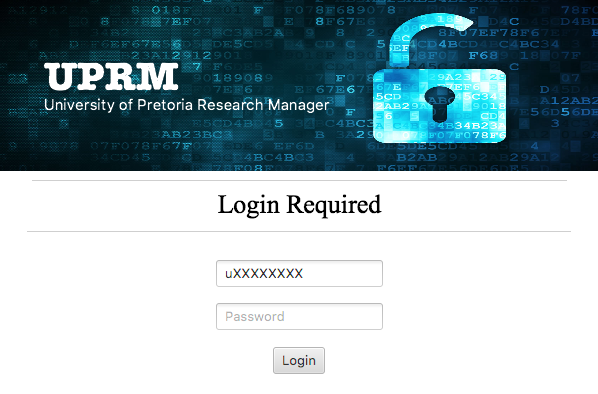
\includegraphics[scale=0.4]{Interfaces/Login.png}}}\\ \\
	\centerline{\fbox{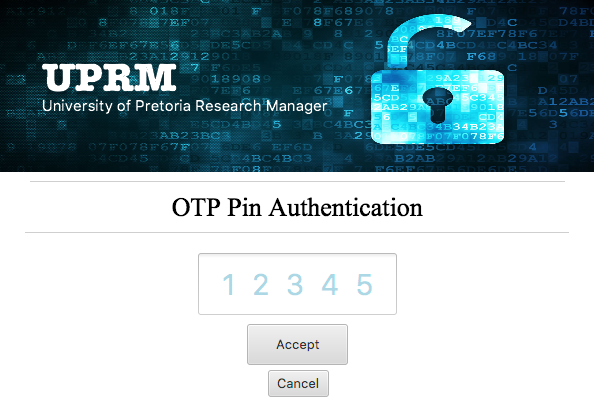
\includegraphics[scale=0.4]{Interfaces/otp.png}}}\\
	
	As soon as the user has entered the correct OTP, then the user will have access to the UPRM system. Once inside the UPRM system they can navigate to any functionality that is available on their user permission level. On the RMSQ the user will be asked to refine a query for their search on statistics of the projects.\\ Some details they could be asked for are as follow:
	\begin{itemize}
		\item Name of a project.
		\item The dates of projects.
		\item The status type of a project.
		\item The specific venue for a project.
		\item A specific author for a project.
	\end{itemize}
	As soon as the user has entered their desired query information, the user will have to be able to choose between displaying the statistics gathered or exporting the report by making use of the RMR functionality.\\ \\
	\textbf{Mockup of a RMSQ interface for the UPRM system: }\\
	\centerline{\fbox{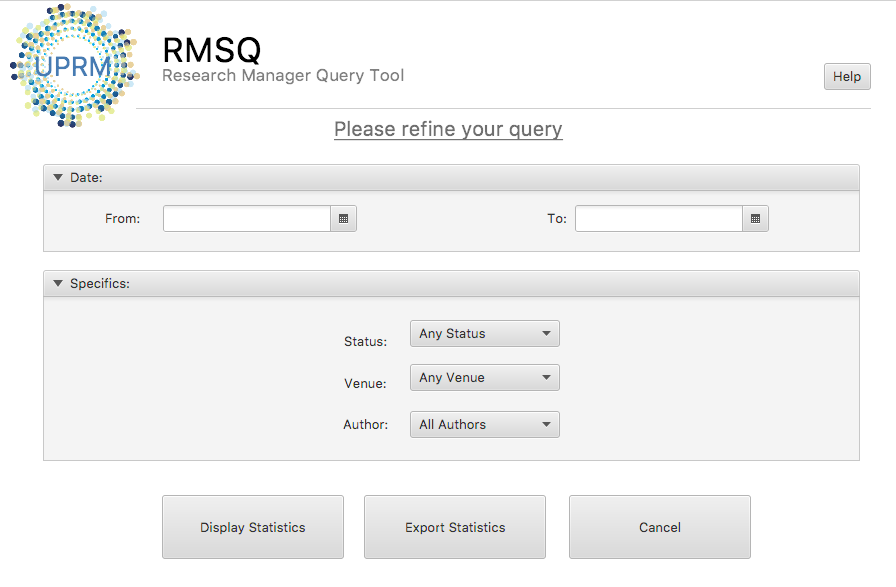
\includegraphics[scale=0.4]{Interfaces/rmsq.png}}}\\ \\
	The RMVC interface will require the user to enter the following information:
	\begin{itemize}
		\item Name of the venue.
		\item Name of the organisation responsible for the venue.
		\item The date for the deadline of submissions, or marking a checkbox to indicate that no deadline exists.
		\item Contact details to which submissions will be sent.
	\end{itemize}
	\pagebreak
	\textbf{Mockup of a RMVC interface for the UPRM system: }\\
	\centerline{\fbox{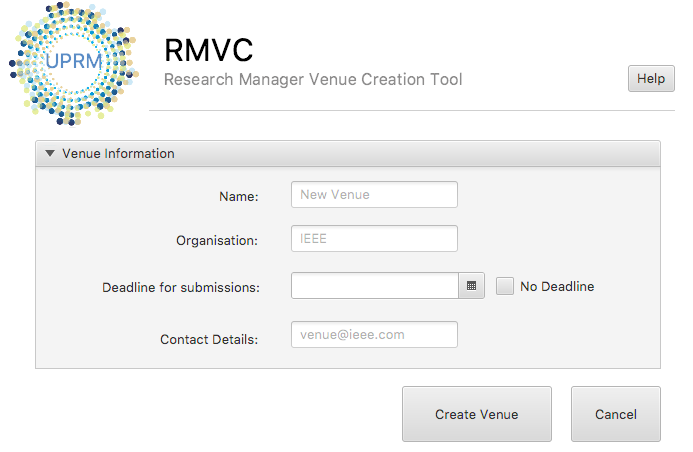
\includegraphics[scale=0.4]{Interfaces/rmvc.png}}}\\
	
	
\subsubsection{Hardware Interfaces}
	As UPRM will only be interfaced through a web portal, UPRM does not have any direct hardware interfaces. UPRM will have a responsive design and will hence work on any physical hardware platform that has an internet connection and a web browser.
	
\subsubsection{Software Interfaces}
	Most of UPRM communication will be with the database system. The communication with the database will consist of reading, writing and modifying data based on the permission levels set by the administrator for that user. The UPRM consist of mainly three software interfaces namely:
	\begin{itemize}
		\item A web server.
		\item A database server.
		\item A client interface.
	\end{itemize}

\subsubsection{Communication Interfaces}
	The communication between the different parts of the system is important since they depend on each
	other. However, in what way the communication is achieved is not important for the system and is
	therefore handled by the underlying operating systems.


	\subsection{Functional Requirements}
		%authentication use case

\subsubsection{Authentication}
UPRM works with sensitive and personal data therefore security plays a massive role in UPRM.
Users will be required to login with a username, password and one-time generated password. UPRM will therefore have build-in two step authentication. \\ \\
A user will be authenticated against LDAP with their username and password. Once LDAP authentication is successful a one-time pin will be generated for the user.\\ \\
Access rights and privileges will be set by an admin user. The admin user will have full access rights and privileges to UPRM.\\ \\
\textbf{Use Cases:}
\begin{itemize}
	\item Register New User
	\item Login
	\item Logout \\
\end{itemize}
\textbf{Authentication Use Case Overview Diagram:}\\
\centerline{\fbox{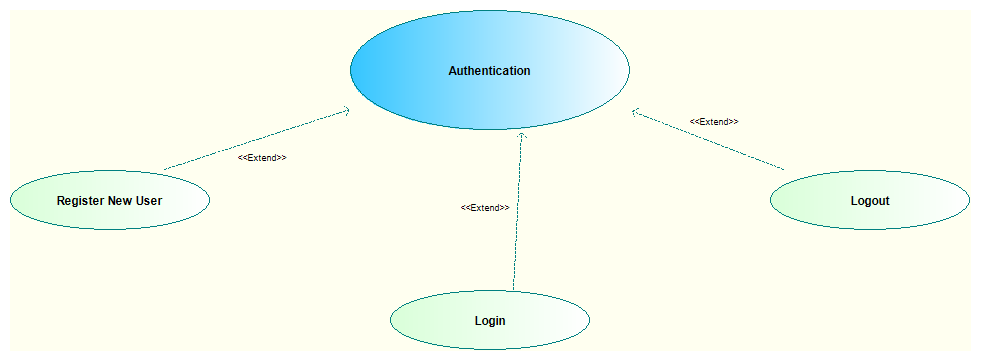
\includegraphics[width=\linewidth]{auth/OverviewAuthUseCase}}}



		\subsubsection{Project}
	In the UPRM system, projects will refer to any new paper or report that the researcher(s) will be involved in. The user has to be able to create multiple projects and keep track of progress by means of a timeline and project specific sub-deadlines.
	The access rights and privileges to each operation will have to be checked before any operation is executed.\\
	\textbf{Use Cases:}
	\begin{itemize}
		\item Creation of Project
		\item Creation of Timeline
		\item Updating of Project
		\item Update of Timeline
		\item Deletion of Project
	\end{itemize}
	\textbf{Project Use Case Overview Diagram:}\\
	\centerline{\fbox{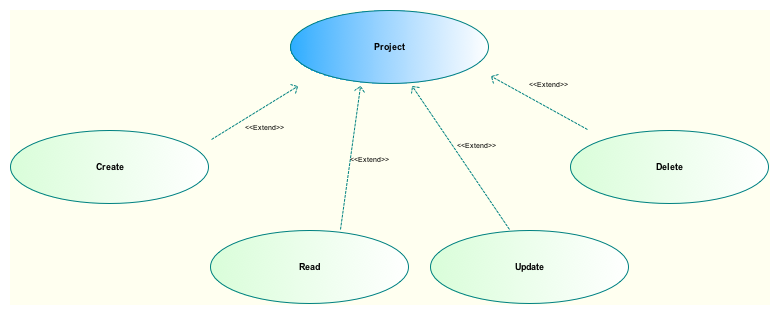
\includegraphics[width=\linewidth]{CRUD/uprm_CRUD_Overview.png}}}		
	
		\subsubsection{Notifications}
Notifications should be via email and standard SMS.\\
Users should be notified of
\begin{itemize}
	\item upcoming deadlines,
	\item changes in the status of a project and
	\item general administration changes.
\end{itemize}


		\subsubsection{Venue}
	The venue selection module will be used by third-party UPRM users and will thus have minimum functionality available. The users should be able to create new venues, update the venues and delete venues.\\
	\textbf{Use Cases:}
	\begin{itemize}
		\item Creation of a venue.
		\item Updating of a venue.
		\item Deletion of a venue.
		\item Sending feedback and updating status to a project.
	\end{itemize}
	\textbf{Venue Use Case Overview Diagram:}\\
	\centerline{\fbox{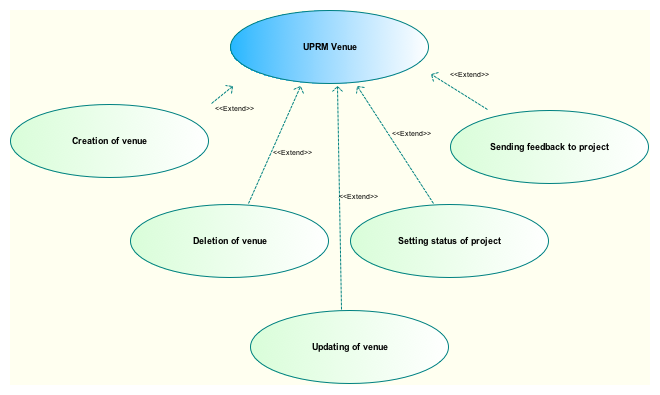
\includegraphics[scale=0.8]{venue/uprm_venueOverview.png}}}	
		\subsubsection{Reporting}
Administrators and General Users should be able to export statistics into known formats, in other words UPRM should generate reports based on selected data.\\ \\
Administrators should be able to generate reports on the data of any number of users, however general users may only generate reports based on data of themselves and not other users.


		\subsubsection{Statistics}
UPRM should be able to display statistics based on specified criteria.\\ \\
Administrators should be able to view any statistics based on the specified criteria. Administrators should be able to view all statistics of all and any general user registered on UPRM. \\ \\
General users may only view statistics of themselves and should be prohibited to view any statistics from another user.
		
	\subsection{Use Cases}
		\subsubsection{Authentication : Register New User}
Administrators and general users will already be registered on UPRM and their details will be stored on the LDAP authentication database.\\ \\
Third party users should be able to register with UPRM to gain access to the system. The details of such a user will be stored in the UPRM database.\\ \\
\textbf{Pre-Conditions}
\begin{itemize}
	\item The user should provide the following information for registration:
	\begin{itemize}
		\item Name,
		\item Surname,
		\item Username,
		\item Email and
		\item Password \\
	\end{itemize}
\end{itemize}
\textbf{Post-Conditions}
\begin{itemize}
	\item User now has access to UPRM.
	\item User details is stored in the UPRM database.\\
\end{itemize}
\textbf{Register New User Use Case Diagram:}\\
\centerline{\fbox{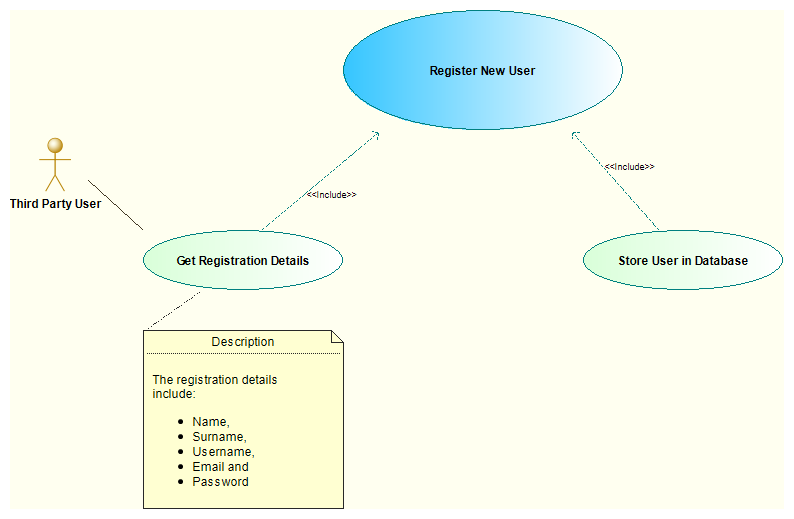
\includegraphics[width=\linewidth]{auth/RegisterNewUser}}}
\subsubsection{Authentication : Login}
Users should be able to login to UPRM.\\
Administrators and General User should be authenticated using LDAP. \\
Third party users should be authenticated using the UPRM database.\\ \\
\textbf{Pre-Conditions}
\begin{itemize}
	\item User should provide the correct username and password.
	\item After receiving the one-time pin the user should provide the system with the correct one-time pin.\\
\end{itemize}
\textbf{Post-Conditions}
\begin{itemize}
	\item If the login was successful,
		\begin{itemize}
			\item a user session should be created and stored.
			\item the user will gain access to UPRM with his/hers specific rights and privileges.
		\end{itemize} 
	\item If the login was not successful,
			\begin{itemize}
				\item the user should be notified of the error that caused the login to be unsuccessful.
				\item the user should have up to 5 tries to login, after which the account will be locked. An administrator should be contacted to unlock the account. \\
			\end{itemize} 
\end{itemize}
\textbf{Login Use Case Diagram:}\\
\centerline{\fbox{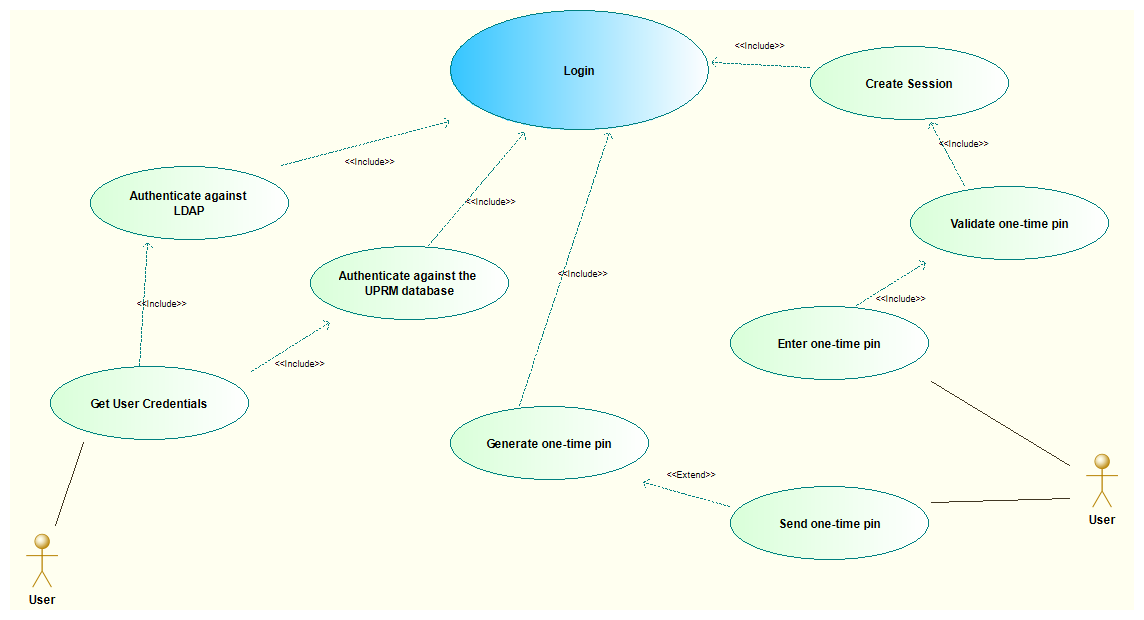
\includegraphics[width=\linewidth]{auth/Login}}}

\subsubsection{Authentication : Logout}
Users should be able to logout of UPRM.\\ \\
\textbf{Pre-Conditions}
\begin{itemize}
	\item User should be logged into UPRM.
	\item A user session should exist.\\
\end{itemize}
\textbf{Post-Conditions}
\begin{itemize}
	\item User not logged into UPRM anymore.
	\item The user session should be removed.\\
\end{itemize}
\textbf{Logout Use Case Diagram:}\\
\centerline{\fbox{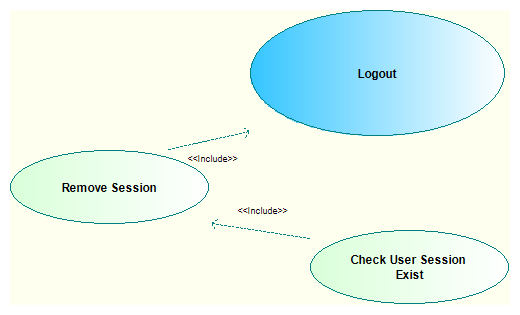
\includegraphics[scale=0.8]{auth/Logout}}}

		\subsubsection{Project : Creating new Projects}
	Once a user has been successfully authenticated by the UPRM system, the user should be able to create a new project.\\ On creation of a new project, the user will have to provide the following details:
	\begin{itemize}
		\item Name(or Title) of the new project.
		\item A short description of the new project.
		\item An overall project deadline.
		\item Optional project specific sub-deadlines to track progress. The default timeline will be from project creation date to overall project deadline and a 1\% progress.\\
	\end{itemize}
	\textbf{Pre-Conditions}
	\begin{itemize}
		\item User has to be successfully authenticated.\\
	\end{itemize}
	\textbf{Post-Conditions}
	\begin{itemize}
		\item A new project should be created.
		\item The new project information should be saved in a database.\\
	\end{itemize}
	\textbf{Use case diagram for creation of projects: }\\
	\centerline{\fbox{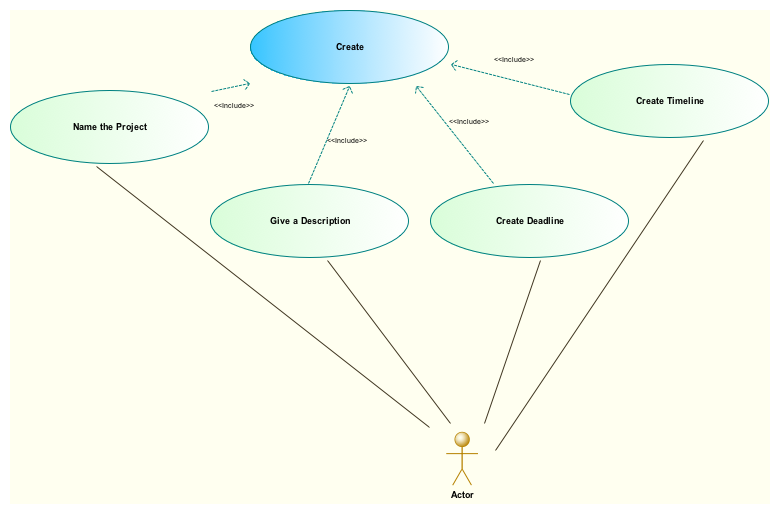
\includegraphics[width=\linewidth]{CRUD/uprm_create.png}}}
	
\subsubsection{Project : Creation of timeline}
	As soon as a project is created, a timeline for that project is also created. This timeline will be used by the statistics module and the users to track the progress of the project.\\ \\
\textbf{Pre-Conditions}
\begin{itemize}
	\item User has to be successfully authenticated.
	\item A project has to exist. \\
\end{itemize}
\textbf{Post-Conditions}
\begin{itemize}
	\item The starting date of the timeline should be saved.
	\item Optional sub-deadlines should be saved.
	\item A progress indicator (defaulting to 1\%) should be updated.\\
\end{itemize}
\textbf{Use case diagram for creation of timelines: }\\
\centerline{\fbox{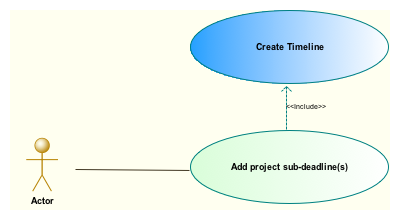
\includegraphics[scale=0.6]{CRUD/uprm_createTimeline.png}}}	
	
\subsubsection{Project : Updating of existing Projects}
	The user should be able to edit the details of an existing project.\\
	 The user will not at any point be able to change the creation date of the project however the details the user will be able to change will be as follow:
	\begin{itemize}
		\item Name(or Title) of the project.
		\item The description of the project.
		\item The optional project specific sub-deadlines for progress tracking. This means adding and removing new sub-deadlines to the timeline.\\
	\end{itemize}
\textbf{Pre-Conditions}
\begin{itemize}
	\item User has to be successfully authenticated.
	\item User has to have the rights/permissions to the particular project.
	\item The project to be updated has to exist. \\
\end{itemize}
\textbf{Post-Conditions}
\begin{itemize}
	\item The project details should be updated.
	\item The project information should be updated in a database.
	\item The progress indicator should be updated.\\
\end{itemize}
\textbf{Use case diagram for updating of projects: }\\
\centerline{\fbox{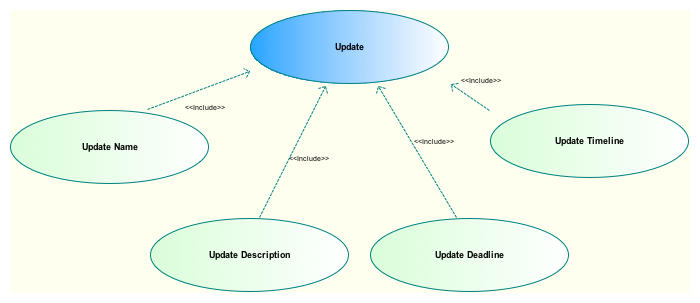
\includegraphics[width=\linewidth]{CRUD/uprm_update.png}}}

\subsubsection{Project : Updating of existing project timeline}
The user should be able to update the timeline of their project at any time. This meaning that the user should be able to add and remove sub-deadlines. This will impact the progress indicator.\\ \\
\textbf{Pre-Conditions}
\begin{itemize}
	\item User should be successfully authenticated.
	\item A project has to exist.
	\item The user should have the rights/permissions to the particular project.
	\item A timeline for the particular project should exist.\\
\end{itemize}
\textbf{Post-Conditions}
\begin{itemize}
	\item The optional sub-deadlines should be updated in the database.
	\item The progress indicator should be updated.\\
\end{itemize}
\pagebreak
\textbf{Use case diagram for updating of timelines: }\\
\centerline{\fbox{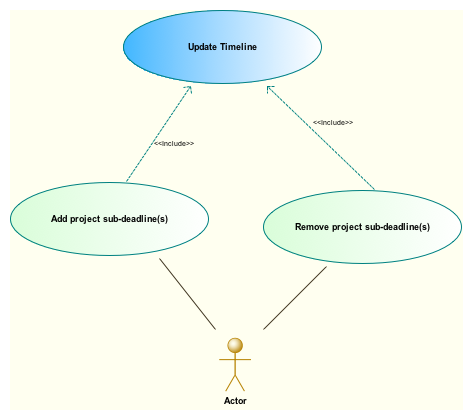
\includegraphics[scale=0.5]{CRUD/uprm_updateTimeline.png}}}

\subsubsection{Project : Deletion of existing project}
A user should be able to discard a project completely at any time. Once the user has chosen to delete a project, the project is completely removed from the UPRM system and all data regarding that project, removed from the UPRM system.\\ \\
\textbf{Pre-Conditions}
\begin{itemize}
	\item User should be successfully authenticated.
	\item A project has to exist.
	\item The user should have the rights/permissions to the particular project.\\
\end{itemize}
\textbf{Post-Conditions}
\begin{itemize}
	\item The particular project information should be deleted from the database.\\
\end{itemize}
\textbf{Use case diagram for deleting of projects: }\\
\centerline{\fbox{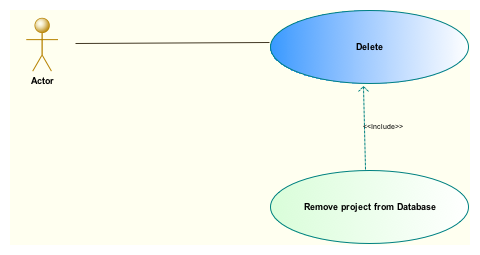
\includegraphics[scale=0.5]{CRUD/uprm_delete.png}}}
		\subsubsection{Notifications}
A user should be notified of
\begin{itemize}
	\item upcoming deadlines,
	\item changes in the status of a project,
	\item password changes,
	\item when a user account was locked,
	\item when the user creates a new project and
	\item any other relevant updates in the user account.
\end{itemize}
\textbf{Pre-Conditions}
\begin{itemize}
	\item User must have valid notification details, such as a mobile number or email address.
\end{itemize}
\textbf{Post-Conditions}
\begin{itemize}
	\item User receive notification with the correct notification event details.
\end{itemize}
\textbf{Diagram:}\\
\centerline{\fbox{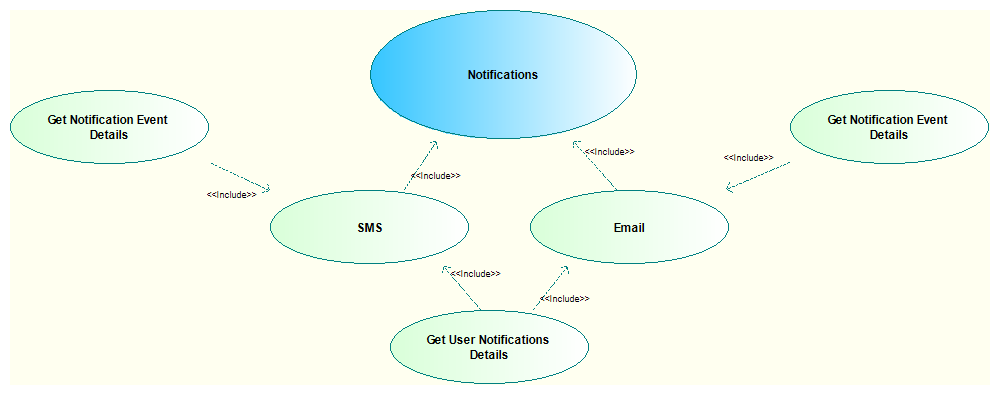
\includegraphics[width=\linewidth]{notifications/Notifications}}}

		\subsubsection{Venue : Creating new venue}
	Once a user has been successfully authenticated by the UPRM system, the user should be able to create a new venue. The venue creation will require the following information before the creation is finalised: 
	\begin{itemize}
		\item Name of the new venue.
		\item The name of the organisation responsible for the venue.
		\item A date signifying the deadline for submissions.
		\item Contact details to where the submissions should be posted (i.e. email address).
	\end{itemize}
	\textbf{Pre-Conditions}
	\begin{itemize}
		\item User has to be successfully authenticated.
	\end{itemize}
	\textbf{Post-Conditions}
	\begin{itemize}
		\item A new venue should be created.
		\item The new venue information should be saved in a database.
	\end{itemize}
	\textbf{Use case diagram for creation of venues: }\\
	\centerline{\fbox{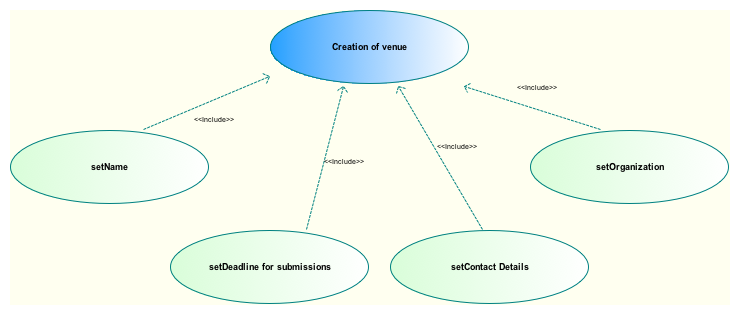
\includegraphics[width=\linewidth]{venue/uprm_venueCreate.png}}}
	
\subsubsection{Venue : Updating venue}
Iff a venue exists and the authenticated user wishes to change some information regarding their venue then the user should be able to do so. The user should be able to change the following information of a venue: 
\begin{itemize}
	\item Name of the venue.
	\item The date signifying the deadline for submissions.
	\item Contact details to where the submissions should be posted (i.e. email address).
\end{itemize}
\textbf{Pre-Conditions}
\begin{itemize}
	\item User has to be successfully authenticated.
	\item The venue should already exist.
\end{itemize}
\textbf{Post-Conditions}
\begin{itemize}
	\item A venue should be updated.
	\item The venue information should be updated in a database.
\end{itemize}
\textbf{Use case diagram for updating of venues: }\\
\centerline{\fbox{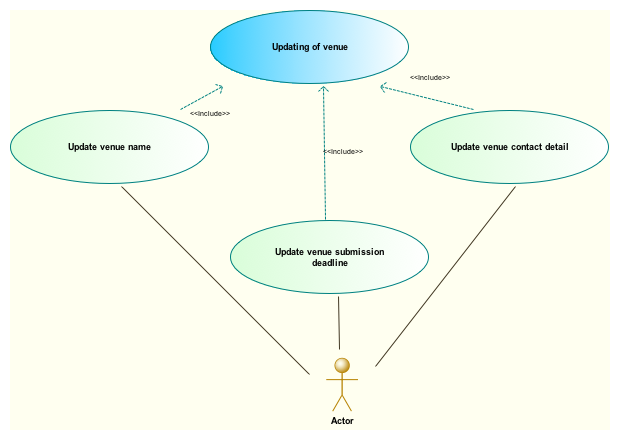
\includegraphics[width=\linewidth]{venue/uprm_venueUpdate.png}}}

\subsubsection{Venue : Deleting venue}
Iff a venue exists and the authenticated user wishes to remove a venue from the UPRM system.
\textbf{Pre-Conditions}
\begin{itemize}
	\item User has to be successfully authenticated.
	\item The venue should already exist.
	\item There should not be any pending submissions.
\end{itemize}
\textbf{Post-Conditions}
\begin{itemize}
	\item The venue should be completely removed from the UPRM database.
\end{itemize}

\subsubsection{Venue : Sending feedback and updating status}
Once a submission is received and has been reviewed by the venue, the venue can send feedback to the project.
\textbf{Pre-Conditions}
\begin{itemize}
	\item User has to be successfully authenticated.
	\item The venue should already exist.
	\item The project should already exist.
\end{itemize}
\textbf{Post-Conditions}
\begin{itemize}
	\item The project feedback information should be updated in the database and a notification sent out.
	\item The status of the project should change.
\end{itemize}
		\subsubsection{Reporting}
Reports should be generated based on the data selection and then be exported to a known format.\\ \\
Formats Include:
\begin{itemize}
	\item PDF
	\item CSV
	\item HTML
\end{itemize}
\textbf{Pre-Conditions}
\begin{itemize}
	\item The user must be logged into UPRM to generate reports.
	\item The user must have the right privileges to be able to export the specific data.
\end{itemize}
\textbf{Post-Conditions}
\begin{itemize}
	\item A report in the specified format should open or be saved on the local computer of the user.
\end{itemize}
\textbf{Diagram:}\\
\centerline{\fbox{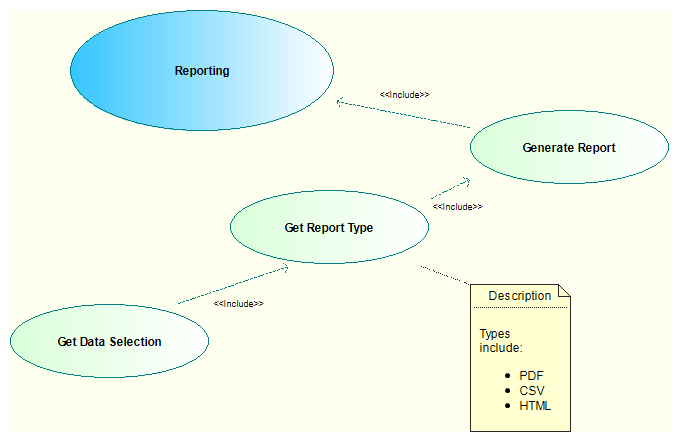
\includegraphics[width=\linewidth]{reporting/Reporting}}}
		\subsubsection{Statistics}
A user should be able to view statistics,
\begin{itemize}
	\item from and to a certain date
	\item for projects with a specific status
	\item for projects done by a specific author or co-author
	\item from which authors collaborated on projects
	\item based on the venue of a project(s)\\
\end{itemize}
More than one criteria should be able to be specified in other words you should be able for example view what the status is of all projects done by a certain author or co-author in a time period.\\ \\
\textbf{Pre-Conditions}
\begin{itemize}
	\item The user should be logged into UPRM.
	\item The user must be a administrator or general user. The user may not be a third party user.
	\item The user must have the right privileges to view the specific data.\\
\end{itemize}
\textbf{Post-Conditions}
\begin{itemize}
	\item Statistics should be displayed in a formatted table with headings.\\
\end{itemize}
\textbf{Statistics Use Case Diagram:}\\
\centerline{\fbox{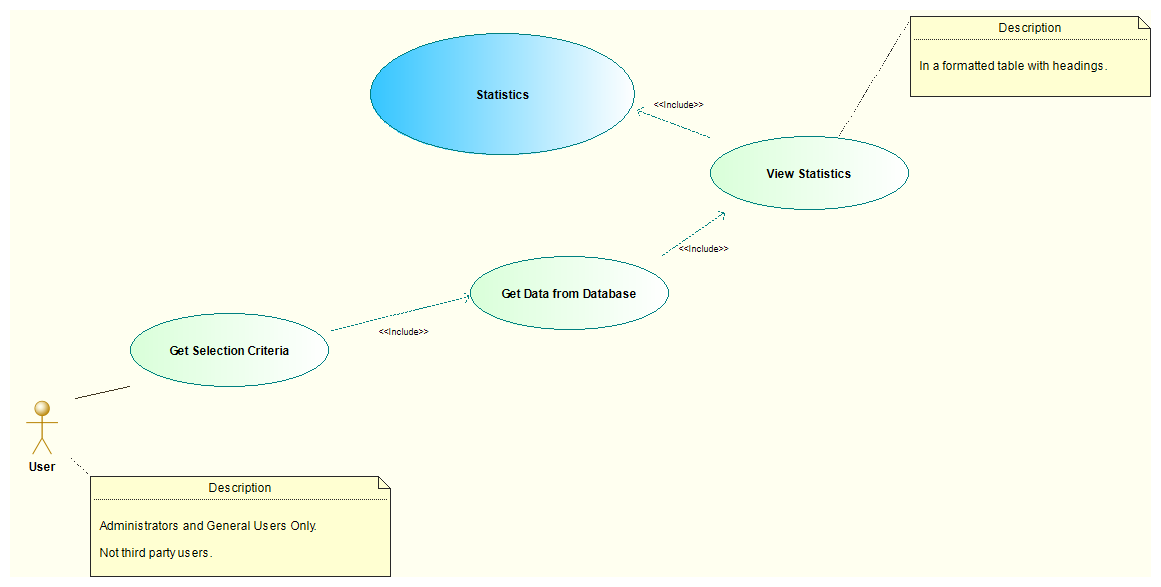
\includegraphics[width=\linewidth]{statistics/Statistics}}}
		
	\subsection{Classes and Objects}
		\subsubsection{Authentication and User}
The authentication class will have login, logout, register user and get session operations. An instance of authentication will hold the current user session.\\ \\
Since third party users should be able to register we need a user class to store the user details. Each private attribute needs a getter function to be able to get the user data for registration.\\ \\
\textbf{Authentication and User Class Diagram:}\\
\centerline{\fbox{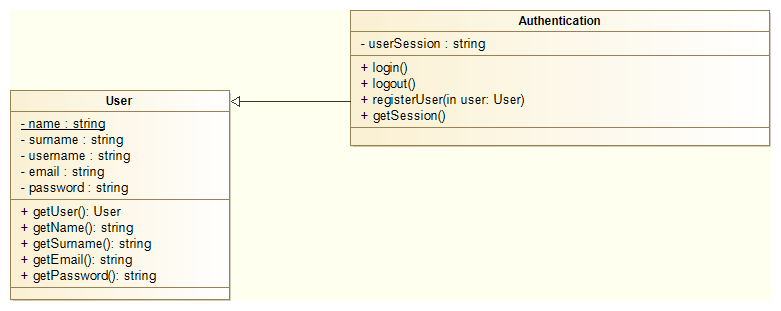
\includegraphics[width=\linewidth]{auth/AuthenticationClassDiagram}}}

		\subsubsection{Project}
A project is the main part of the UPRM system and hence a very important class to implement. The class should have no default constructor and should always create a new Timeline object in the parameterized constructor.\\ \\
\textbf{Project Class Diagram:}\\
\centerline{\fbox{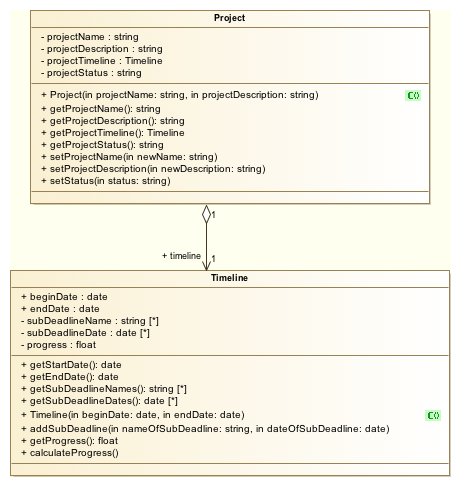
\includegraphics[scale=0.6]{CRUD/ProjectClassDiagram.png}}}
		\subsubsection{Notifications}
UPRM should utilise two different notification techniques namely email and sms. A Strategy Design Pattern should be implemented to enable more notifications to be added on a later stage and to enable a user to choose between different notification types.\\ \\
\textbf{Notifications Class Diagram:}\\
\centerline{\fbox{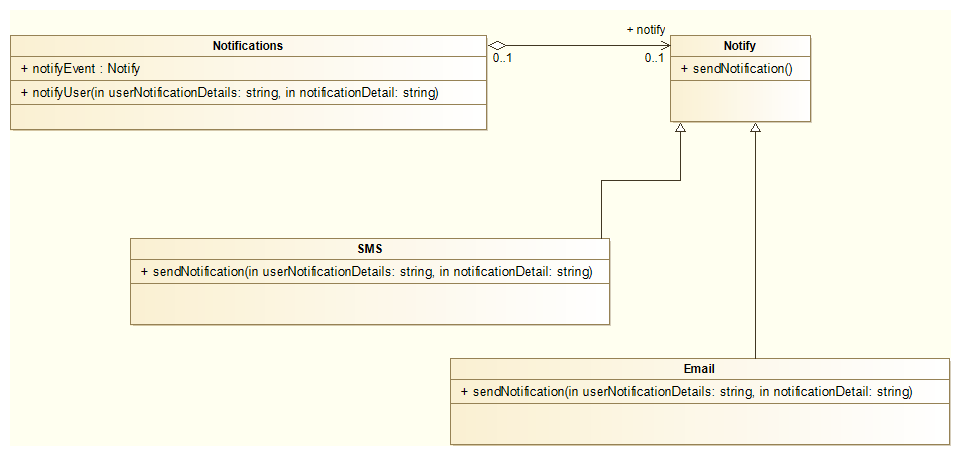
\includegraphics[width=\linewidth]{notifications/NotificationsClassDiagram}}}
		\subsubsection{Venue}
A venue will have to have a contact detail field and it could be of a certain type. Hence we make use of the strategy pattern and enable the user to add any type of contact information, that UPRM supports, to which submissions will be sent. How the Contact class is structured will be up up for the developer to choose.\\ \\
\textbf{Venue Class Diagram:}\\
\centerline{\fbox{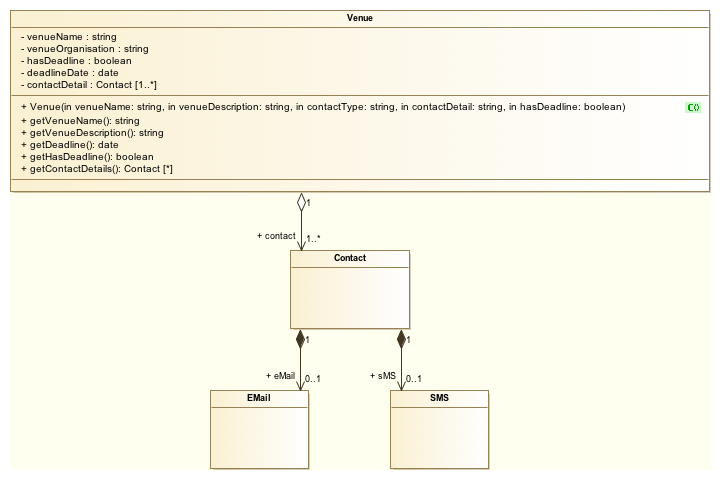
\includegraphics[width=\linewidth]{venue/venue_class_diagram.png}}}
		\subsubsection{Reporting}
The reporting class should have an operation to get the report type from the user, an operation to generate the report. The class should have operations to display and save the report.\\ \\ 
\textbf{Reporting Class Diagram:}\\
\centerline{\fbox{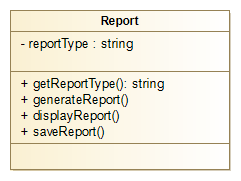
\includegraphics[scale=0.8]{reporting/ReportingClassDiagram}}}



		\subsubsection{Statistics}

\textbf{Statistics Class Diagram:}\\
\centerline{\fbox{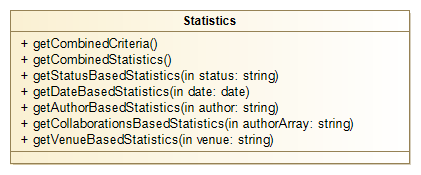
\includegraphics[scale=0.8]{statistics/StatisticsClassDiagram}}}





	\subsection{Non-Functional Requirements}
		%nonfunctional
% We have to decide on the utmost important req here and remove the others

\subsubsection{Performance}
For UPRM performance will not be a core non-functional requirement, however to make the system feasible and usable the following requirements must hold:

\begin{itemize}
	\item The response time of any query should be \textless{}  5 seconds.
	\item The generation of any report or statistic should be at most 10 seconds.
\end{itemize}

\subsubsection{Reliability}
Any system that works with live data such as UPRM should be reliable to ensure the integrity of the data stored in the database.\\
 
The following requirements must therefore hold, UPRM 

\begin{itemize}
	\item should never crash while updating, creating or removing research projects.
	\item should perform any functionality as precise as specified in the functional requirements at any moment during the use of the system.
\end{itemize}

\subsubsection{Availability}
Availability is a crucial non-functional requirement as the updating and creating of research projects is the most important requirement of UPRM.\\

Availability requirements are as follows,

\begin{itemize}
	\item UPRM have to be in a functional and working state for 95 - 99\% of the time per year. Downtime will then be between 3.45 - 18.25 days per year.
	\item UPRM may not exceed a continuous downtime for longer than 3 hours.
	\item MTTF of UPRM may not exceed 30 seconds.
\end{itemize}

\subsubsection{Security}
Security is one of the most significant non-functional requirements as the data that is processed and stored by UPRM is of a sensitive nature. 
A vast amount of research ideas and the progress status on current research will be stored by UPRM needless to say, if such data falls into the wrong hands it could jeopardise the research project or the idea of the research.\\ 

\textbf{In terms of security}, UPRM should,
	\begin{itemize} 
		\item never reveal the current progress of research projects to unauthorized parties.
		\item never reveal future research ideas to unauthorized parties.
		\item prevent the loss of any data (personal and research related data).
	\end{itemize}

\textbf{In terms of security requirements}, UPRM should,
	\begin{itemize} 
		\item make use of strong passwords.
		\item utilise two step verification/authentication.
		\item make sure that password resets is done by an administrator.
	\end{itemize}

\subsubsection{Maintainability}

\subsubsection{Portability}

	\subsection{Inverse Requirements}


	\subsection{Design Constraints}


	\subsection{Logical Database Requirements}


	\subsection{Other Requirements}
	\pagebreak

	%analysismodels
%If we have such models or feel the need to add it, we can
\section{Analysis Models}
	
	\subsection{Sequence Diagrams}
	\subsection{Activity Diagrams}


	\section{Change Management Process}
	This requirements documentation will be updated every time the requirements change whether its a change from the development team or the client. Everyone in the development team will have the right to change the requirements document with the team leader approving the change and ultimately the client approving major changes.

	\pagebreak

	%appendices

\section{Appendices}

	\subsection{Appendix 1}
	\subsection{Appendix 2}
	\subsection{Appendix 3}

	
\end{document}